% \documentclass[german,master,buw]{webisthesis} % Weimar
\documentclass[english,bachelor,fsu]{webisthesis} % Jena
% \documentclass[german,bachelor,ul]{webisthesis} % Leipzig
% \documentclass[german,master,buw,web]{webisthesis} % Weimar, for web page
% \documentclass[german,bachelor,fsu,web]{webisthesis} % Jena, for web page
% \documentclass[german,bachelor,ul,web]{webisthesis} % Leipzig, for web page
%
% Non-default programme
% ---------------------
% \documentclass[english,master,buw]{webisthesis}\global\thesisprogramme{Human-Computer Interaction}
% \documentclass[english,master,buw]{webisthesis}\global\thesisfrontpagefaculty{Faculty of Civil Engineering/Faculty of Media}\global\thesisprogramme{Digital Engineering}
% \documentclass[german,bachelor,buw]{webisthesis}\global\thesisprogramme{Informatik\\Schwerpunkt Medieninformatik}
% \documentclass[german,bachelor,buw]{webisthesis}\global\thesisprogramme{Informatik\\Schwerpunkt Security and Data Science}
%
% When you change the language, pdflatex may halt on recompilation.
% Just hit enter to continue and recompile again. This should fix it.


%
% Values
% ------
\ThesisSetTitle{Analyzing Toxicity on Mastodon}
\ThesisSetKeywords{These, are, my, Keywords} % only for PDF meta attributes
\ThesisSetLocation{Jena} 

\ThesisSetAuthor{Julian Klüber}
\ThesisSetStudentNumber{201071}
\ThesisSetDateOfBirth{8}{7}{2001}
\ThesisSetPlaceOfBirth{Hünfeld}

% Supervisors should usually be Professors from the candidate's university. A second supervisor is not always needed. 
\ThesisSetSupervisors{Prof.\ Dr.\ Hagen}

\ThesisSetSubmissionDate{16}{04}{2025}

\usepackage{graphicx}
\usepackage{tabularx}

%
% Suggested Packages
% ------------------
\usepackage[sort&compress]{natbib}
%   Allows citing in different ways (e.g., only the authors if you use the
%   citation again within a short time).
%
\usepackage{booktabs}
%    For tables ``looking the right way''.
%
% \usepackage{tabularx}
%    Enables tables with columns that automatically fill the page width.
%
% \usepackage[ruled,algochapter]{algorithm2e}
%    A package for pseudo code algorithms.
%
% \usepackage{amsmath}
%    For tabular-style formatting of mathematical environments.
%

\usepackage{fontawesome}
%    For lots of awesome glyphs: https://mirror.physik.tu-berlin.de/pub/CTAN/fonts/fontawesome/doc/fontawesome.pdf

%
% Commenting (by your supervisor)
% -------------------------------
\usepackage{xcolor}
\usepackage{soul}
\newcommand{\bscom}[2]{%
  % #1 Original text.
  % #2 Replacement text.
    \st{\scriptsize\,#1}{\color{blue}\scriptsize\,#2}%
  }

% Create links in the pdf document
% Hyperref has some incompatibilities with other packages
% Some other packages must be loaded before, some after hyperref
% Additional options to the hyperref package can be provided in the braces [], like in
% \usehyperref[backref] % This will add back references in the bibliography that some people like ... some don't ... so better ask your supervisor ;-)
\usehyperref

\begin{document}
\begin{frontmatter}
\begin{abstract}
\end{abstract}

\tableofcontents

% \chapter*{Acknowledgements} % optional
% I thank the authors of the webisthesis template for their excellent work!

% \listoffigures % optional, usually not needed

% \listoftables % optional, usually not needed

% \listofalgorithms % optional, usually not needed
%    requires package algorithm2e

% optional: list of symbols/notation (e.g., using the nomencl package) but usually not needed
\end{frontmatter}

\chapter{Introduction}\label{introduction}

% Social media has become an essential part of modern life, enabling billions of people to share their stories, connect over shared interests, and participate in discussions on global events. This has resulted in the formation of large online communities. Unlike physical communities, online communities allow for easier and more immediate grouping of individuals, as joining a community often requires minimal effort; simply clicking a button or following a page \cite{ellison:2007}. This ease of access fosters the creation of diverse and dynamic social ecosystems, where users interact under shared norms, behaviors, and communication styles unique to each community.

% However, the aggregation of large numbers of individuals in online communities also increases the likelihood of negative behaviors, such as toxicity. Toxicity in online spaces refers to harmful actions, including hate speech, racism, sexism, and other forms of discrimination \cite{fan:2022}. These behaviors are often exacerbated by the anonymity and reduced social inhibitions that characterize digital environments \cite{suler:2004,moore:2012,wulczyn:2016}.

Social media platforms reinforce the risk of toxic behavior, such as hate speech, harassment, and discrimination, compared to traditional media, due to their scale, anonymity, and minimal barriers to community entry \cite{fan:2022,suler:2004,ellison:2007}. While these platforms enable billions to connect and share opinions, their design encourages environments where harmful actions thrive. For instance, the ease of joining online communities (often just a click away) encourages rapid aggregation of users \cite{ellison:2007} but also decreases the sense of responsibility, as anonymity reduces social inhibitions \cite{moore:2012,suler:2004,wulczyn:2017}. This dynamic creates fertile ground for toxicity, which spreads easier in digital spaces than in physical interactions \cite{suler:2004}.

\begin{figure}[tb]
  \centering
  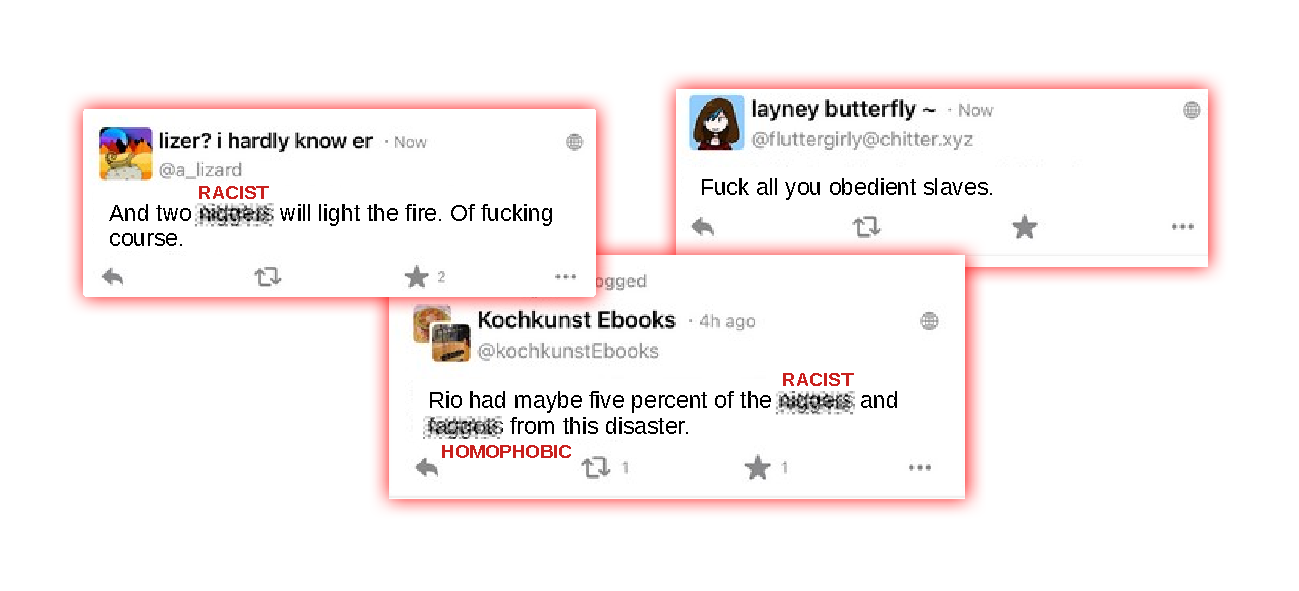
\includegraphics[width=\linewidth]{../material/toxic_comments.pdf}
  \caption{Three toxic examples posted during the 2024 Paris Olympics opening ceremony on Mastodon. The toots shown here contain real content but have been recreated and do not show the real user.}
  \label{toxic-comments}
\end{figure}

Behaviors, like those you can see in Figure\ref{toxic-comments} disrupt community solidarity and harm individual users, making toxicity a significant challenge for social media platforms \cite{fan:2022,wulczyn:2017}. To mitigate these issues, online communities establish rules and moderation systems to enforce acceptable behavior. Violations of these rules can result in penalties, such as bans or restrictions, depending on the platform's moderation policies \cite{nicholson:2023}.

\begin{figure}[tb]
  \centering
  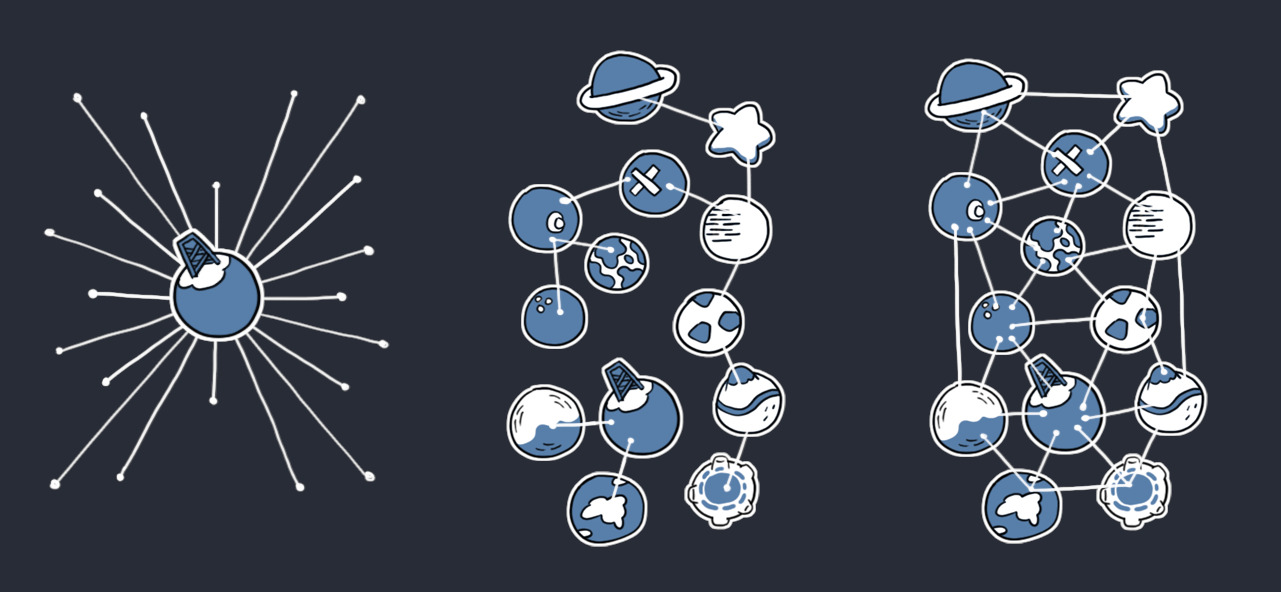
\includegraphics[width=\textwidth]{../material/network_models.jpg}
  \caption{From left to right: Centralized networks connect all through a single controlling hub; Federated networks organize nodes into semi-autonomous interconnected clusters; Distributed networks connect all nodes with multiple pathways \cite{mastodon:docs}.}
  \label{network-models}
\end{figure}

To understand the dynamics of toxicity in online communities and the challenges they face, this case study focuses on Mastodon\footnote{\url{https://mastodon.social/explore}}, a decentralized alternative to traditional social media platforms like Twitter/X\footnote{\url{https://x.com/}}. The recent acquisition of Twitter/X by Elon Musk has highlighted the risks of centralized social media, where a single individual or entity can exert significant control over platform governance, content moderation, and user experience \cite{he:2023}. Such centralization can lead to abrupt policy changes, increased misinformation, and heightened toxicity, prompting users to seek alternatives. Mastodon, as a decentralized and federated platform, offers a contrasting model where power is distributed across independently operated instances. In common with other social media platforms, Mastodon offers the possibility to interact with other people by publishing posts, reacting to posts, or sharing posts. However, Mastodon as a federated social media platform belongs to the decentralized online social networks (DOSNs). Federation refers to a special kind of decentralization explained in Figure~\ref{network-models}. Traditional social media platforms, such as Twitter/X, Facebook, or Instagram, have a single central service that all users access. In contrast, Mastodon has multiple services, called instances, which are used by any number of people. These instances can communicate with each other and create a federated network. Users can freely choose an instance based on language, community rules, moderation policies, and topics of interest. Each instance is managed by its own administrators, who set and enforce local rules \cite{mastodon:docs}. However, this decentralization also introduces unique challenges, such as inconsistent moderation standards and the potential for fragmentation within the fediverse \cite{he:2023}. By examining Mastodon, this study aims to explore how decentralized platforms address toxicity and community management while navigating the complexities of a federated ecosystem.

\paragraph{Research Gap and Contribution}
Prior work has established foundational knowledge about Mastodon's structure \cite{zulli:2020,la_cava:2021}, moderation practices \cite{bono:2024,nicholson:2023}, and toxicity analysis methods \cite{fan:2022}. However, only a few studies have systematically examined toxicity patterns across the entire Mastodon network and those are limited on small datasets, such as the study by \citet{al-khateeb:2022}. Our research addresses this gap by conducting a large-scale toxicity analysis of Mastodon. We analyzed a 1\% subsample of 1.8~billion Mastodon posts (called ``toots'') across 1,000~instances collected throughout 2024. The results reveal two key findings: First, toxicity levels show clear spikes during major political and global events, particularly around the U.S.~election period. Second, active moderation practices seem to lower mean toxicity levels on instances, demonstrating the effectiveness of decentralized moderation approaches.

\enlargethispage{\baselineskip}
\chapter{Related Work}

Research on online toxicity has primarily focused on centralized social media platforms like Twitter/X and Facebook \cite{fan:2022,nicholson:2023}. These studies have examined various aspects of toxic behavior, including its diffusion patterns, impact on communities, and moderation strategies. However, DOSNs like Mastodon present unique challenges and opportunities for studying toxicity due to their federated architecture and distributed moderation systems \cite{bono:2024}. This chapter reviews relevant literature on Mastodon communities, decentralized moderation, and large-scale toxicity analysis to situate our research within the existing work.

\paragraph{Behaviour of Mastodon Communities}
Mastodon has emerged as a prominent DOSN, offering an alternative to centralized platforms by enabling users to join independent instances that form a federated network \cite{zulli:2020}. This setup allows researchers to study community behaviors, particularly how users interact or segregate across instances while this is not possible on centralised platforms \cite{zignani:2018,zulli:2020}.

The topology of Mastodon communities exhibits unique characteristics. \citet{zulli:2020} found that Mastodon instances often form around specific interests, identities, or ideologies, leading to more homogeneous communities. This clustering behavior influences information consumption patterns and user relationships, with instances developing distinct footprints based on their thematic focus \cite{la_cava:2021}. Such organizational differences suggest that toxicity patterns in Mastodon may follow different dynamics than those observed in centralized platforms.

\paragraph{Decentralized Moderation Challenges}
The federated nature of Mastodon introduces novel challenges for content moderation, as each instance maintains its own policies and enforcement mechanisms. \citet{bono:2024} found that instance administrators primarily rely on blocklisting to moderate content, preventing users from interacting with servers hosting harmful material. This decentralized approach allows for customized moderation but creates inconsistencies across the network, as blocklisting decisions vary a lot between instances \cite{nicholson:2023}. \citet{nicholson:2023} found that blocklists mainly ban instances containing spam, hate speech, or adult content. Many administrators use shared blocklists without carefully checking them first \cite{bono:2024}.

\citet{nicholson:2023} examined Mastodon's rules and discovered they focus more on preventing harassment and hate speech than similar Reddit communities. Their research showed that Mastodon's decentralized approach creates different types of rules across instances. Some instances employ rules to target specific toxic behaviour such as discrimination, while others use general community guidelines. Since each instance has its own moderation approach, users see and experience different content depending on which instance they join, making it difficult to investigate toxicity.

\paragraph{Large-Scale Toxicity Analysis}
Existing approaches to toxicity analysis have typically focused on specific events or short timeframes on centralized platforms \cite{wulczyn:2017, fan:2022,georgakopoulos:2018,badjatiya:2017}. For example, \citet{fan:2022} developed a comprehensive workflow for analyzing toxicity during health crises, combining topic modeling and network analysis to understand toxic discourse patterns. Their approach, which processed over 1.6 million tweets during the 2022 Mpox outbreak, revealed how toxicity spreads differently through mentions versus retweets and identified influential users in toxic discourse networks. As a first step toward analyzing toxicity on Mastodon, \citet{al-khateeb:2022} predicted the toxicity of 13,590~toots using the Perspective~API. The scale and distributed nature of Mastodon data require specialized processing pipelines. Existing research has highlighted the need for efficient deduplication methods when analyzing federated content, as toots often propagate across multiple instances \cite{bono:2024}.
\chapter{Dataset} \label{dataset}

\chapter{Choosing Transformer Model} \label{choosing-transformer-model}

To predict the toxicity of the post content, I evaluated three transformer-based models: Detoxify (Original), Detoxify (Unbiased) from Unitary, and Perspective API. These models predict the probability of six to seven toxicity categories.

\section{Annotation} \label{annotation}

All models were evaluated on a specific subset of the dataset. The selected timeframe was the evening of the Olympic Games' opening ceremony, chosen due to the expectation of heightened online discussions and, consequently, an increased presence of toxic content. The dataset covers the period from 20:00 to 23:00 on July 26, 2024, comprising 1,179,897 posts. This context switch which may impact the model performance, but as well shows the model's robustness in a new context.

After the models completed their predictions, a sample was drawn for each model, selecting 25 posts per toxicity category with a predicted probability greater than 0.5 for that category. The selected posts were then concatenated, and duplicates were removed, resulting in a final annotation dataset of 253 posts.

The annotation process was conducted by two researchers using Label Studio. The posts were labeled according to the following categories in the table below. The annotation of hate speech remains a highly subjective task, influenced by individual annotator biases, further affecting consistency and reliability. To ensure the reliability of the annotations, inter-annotator agreement was measured using Cohen's Kappa. The results showed perfect agreement (Cohen's Kappa = 1.0) for the categories of toxic, severe toxic, threat, insult, and identity attack. Near-perfect agreement was achieved for obscene (Cohen's Kappa = 0.9907) and sexually explicit (Cohen's Kappa = 0.9735), indicating a high level of consistency between the annotators.

\begin{table}[h]
    \centering
    \renewcommand{\arraystretch}{1.3}
    \begin{tabularx}{\textwidth}{lX}
        \toprule
        \textbf{Category} & \textbf{Description} \\
        \midrule
        TOXIC & A rude, disrespectful, or unreasonable comment that is likely to make someone leave a discussion. \\
        SEVERE TOXIC & A very hateful, aggressive, or disrespectful comment that is highly likely to push someone away. \\
        IDENTITY ATTACK & Negative or hateful comments targeting someone because of their identity. \\
        INSULT & Insulting, inflammatory, or negative comments towards a person or group. \\
        OBSCENE & Swear words, curse words, or other obscene or profane language. \\
        THREAT & Describes an intention to inflict pain, injury, or violence against an individual or group. \\
        SEXUALLY EXPLICIT & Genital nudity or descriptions of simulated or actual sexual acts. \\
        \bottomrule
    \end{tabularx}
    \caption{Toxicity Categories and Their Descriptions}
\end{table}

\section{Evaluation} \label{evaluation}

In the evaluation of the toxicity detection models, the analysis focused on the probability distributions of toxicity categories across three models: the Perspective API and two Detoxify models (original and unbiased). The evaluation did not involve optimizing prediction thresholds; instead, a fixed threshold of 0.5 was used to compare the F1 scores. The results indicated that the Perspective API model generally outperformed the Detoxify models in terms of F1 score across most toxicity categories. However, a closer examination of the probability distributions revealed notable differences in the models' behavior. The Perspective API model exhibited a widely spread probability distribution, suggesting a more cautious and less confident approach to predictions. In contrast, the Detoxify models demonstrated a more concentrated probability distribution, indicating higher confidence in their predictions.

\begin{figure}[h]
    \centering
    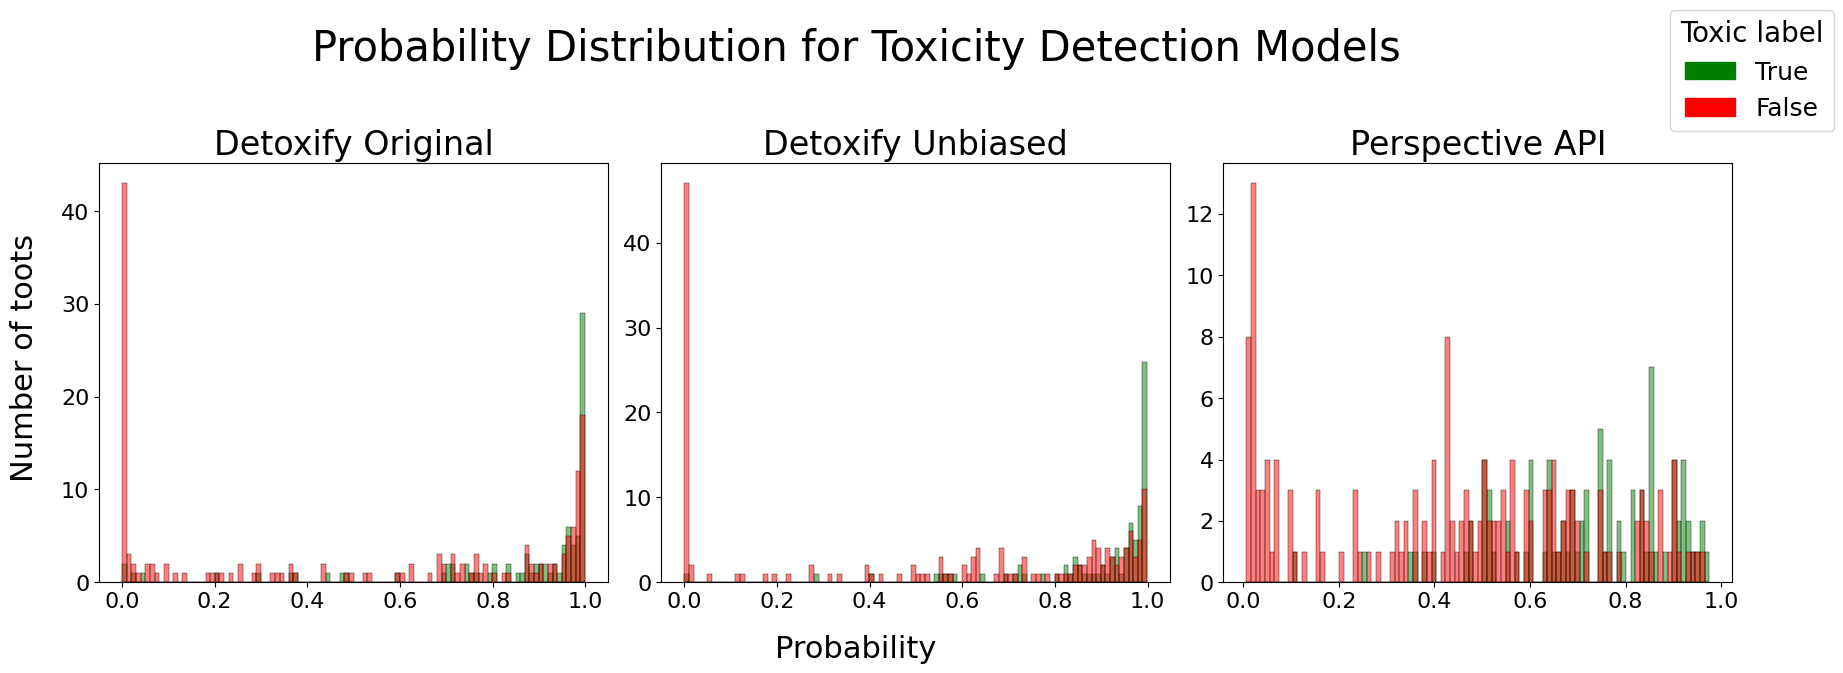
\includegraphics[width=\textwidth]{../material/probability_distribution.png}
    \caption{Probability Distribution of Toxicity category across the three models}
    \label{fig:probability-distribution}
\end{figure}

While the Perspective API model's performance metrics were stronger, its limited accessibility, restricted by a low request rate and lack of open access, posed significant practical limitations for large-scale analysis. On the other hand, the Detoxify models, being open-source, offered unrestricted usage, making them more suitable for extensive studies. Given that the primary objective of this research is not to predict toxicity in individual posts but to analyze broader trends in toxicity across Mastodon instances, the Detoxify models were considered more appropriate. A confident model, such as Detoxify, is better suited for identifying and tracking trends over time.

Between the two Detoxify models, the unbiased version was selected for further analysis due to its superior performance and the inclusion of an additional category, "sexual explicit," which is absent in the original Detoxify model. However, it is important to note that the "severe toxic" label in the Detoxify unbiased model demonstrated poor performance, likely due to the limited number of supporting posts (only 10 in the dataset). Consequently, findings related to this category should be interpreted with caution. Despite this limitation, the Detoxify unbiased model was chosen as the most suitable tool for analyzing toxicity trends in Mastodon communities, balancing performance, accessibility, and practical applicability.


\begin{table}[h!]
\centering
\begin{tabular}{|l|l|c|c|c|c|}
\hline
\textbf{Model} & \textbf{Category} & \textbf{F1} & \textbf{Precision} & \textbf{Recall} & \textbf{Support} \\
\hline
Detoxify Original & & 0.622 & 0.482 & 0.878 & 90 \\
Detoxify Unbiased & toxic & 0.635 & 0.473 & 0.967 & 90 \\
Perspective API & & \textbf{0.664} & 0.526 & 0.900 & 90 \\
\hline
Detoxify Original & & 0.148 & 0.118 & 0.200 & 10 \\
Detoxify Unbiased & severe toxic & 0.000 & 0.000 & 0.000 & 10 \\
Perspective API & & \textbf{0.222} & 0.176 & 0.300 & 10 \\
\hline
Detoxify Original & & \textbf{0.741} & 0.613 & 0.936 & 78 \\
Detoxify Unbiased & obscene & 0.739 & 0.642 & 0.872 & 78 \\
Perspective API & & 0.738 & 0.615 & 0.923 & 78 \\
\hline
Detoxify Original & & 0.462 & 0.429 & 0.500 & 18 \\
Detoxify Unbiased & threat & 0.520 & 0.406 & 0.722 & 18 \\
Perspective API & & \textbf{0.596} & 0.483 & 0.778 & 18 \\
\hline
Detoxify Original & & 0.377 & 0.312 & 0.476 & 42 \\
Detoxify Unbiased & insult & \textbf{0.500} & 0.378 & 0.738 & 42 \\
Perspective API & & 0.487 & 0.384 & 0.667 & 42 \\
\hline
Detoxify Original & & 0.440 & 0.314 & 0.733 & 15 \\
Detoxify Unbiased & identity attack & \textbf{0.545} & 0.414 & 0.800 & 15 \\
Perspective API & & 0.456 & 0.310 & 0.867 & 15 \\
\hline
Detoxify Original & & 0.000 & 0.000 & 0.000 & 21 \\
Detoxify Unbiased & sexually explicit & 0.392 & 0.333 & 0.476 & 21 \\
Perspective API & & \textbf{0.576} & 0.447 & 0.810 & 21 \\
\hline
\end{tabular}
\caption{Performance Metrics with Highlighted Highest F1 Scores}
\end{table}

\section{Detoxify Unbiased} \label{detoxify-unbiased}

The Unbiased Detoxify model is built on the RoBERTa-base architecture, which is a robust transformer model trained specifically for toxicity classification tasks. It was trained using the Jigsaw Unintended Bias in Toxicity Classification Challenge dataset, which includes labeled data for both general toxicity and toxicity directed toward specific identity groups. This makes it a critical tool in distinguishing between harmful general toxic language and toxic language targeting vulnerable identities, such as race, gender, and religion.

The model utilizes a combined loss function during training, which incorporates both toxicity and identity labels. This ensures that the model learns to minimize unintended bias, especially in cases where comments contain identity-related toxicity. A bias metric is also employed to evaluate how well the model performs across various identity subgroups, with the aim of reducing unfair bias in its predictions. \citep{detoxify:medium}
\chapter{Large-Scale Toxicity Analysis} \label{large-scale-analysis}
Having chosen the detoxify unbiased model, we then use a large-scale pipeline to assign seven toxicity values between 0 and 1 to each toot for further analysis. Afterwards we conduct a temporal analysis of toxicity trends across all of 2024. Our investigation further explored the impact of moderation policies and instance rules on average toxicity levels.

\section{Large-Scale Pipeline Architecture}
The pipeline is built using the Ray framework \cite{moritz:2018}, a distributed computing system that simplifies parallel and batch processing of large-scale data workloads. Ray provides high-level APIs for task scheduling and resource management, making it particularly suitable for batch-oriented data processing pipelines. The framework's ability to scale computations across clusters while maintaining fault tolerance makes it ideal for our large-scale toxicity analysis. Our pipeline consists of several stages: data reading, deduplication, toxicity prediction, and merging (Figure~\ref{fig:pipeline}), all efficiently coordinated through Ray's distributed execution model.

\paragraph{Prerequisites}
The Ray environment is configured with specific settings for parallelism, memory, and number of CPU's per task to ensure efficient processing of large datasets. We ran the tasks seperatly in parallel pipelines to avoid memory conflicts and cache our results between the stages. The pipeline is designed to run on a cluster with 507 CPU cores, 976GB of RAM, and 290GB of object store memory, by using 0.01 CPU cores per task, with a maximum of 100 tasks running in parallel. To ensure robustness, the pipeline is configured to retry failed tasks up to 10 times, with retry exceptions enabled to handle briefly flashing errors well. These settings ensure that the pipeline can handle large datasets efficiently on our cluster while minimizing resource conflicts.

For scalability, we used Ray's parallelized datasets\footnote{\url{https://docs.ray.io/en/latest/data/data.html}} and pandas\footnote{\url{https://pandas.pydata.org/docs/user\_guide/index.html}} data frames. The \textit{map\_batches}\footnote{url{https://docs.ray.io/en/latest/data/api/doc/ray.data.Dataset.map\_batches.html}} operation processes data in manageable chunks, distributing the workload across available cluster resources. Each batch is converted to a pandas DataFrame, enabling us to utilise pandas' rich ecosystem of vectorized operations and transformations on each subset of data.

\begin{figure}[tb]
    \centering
    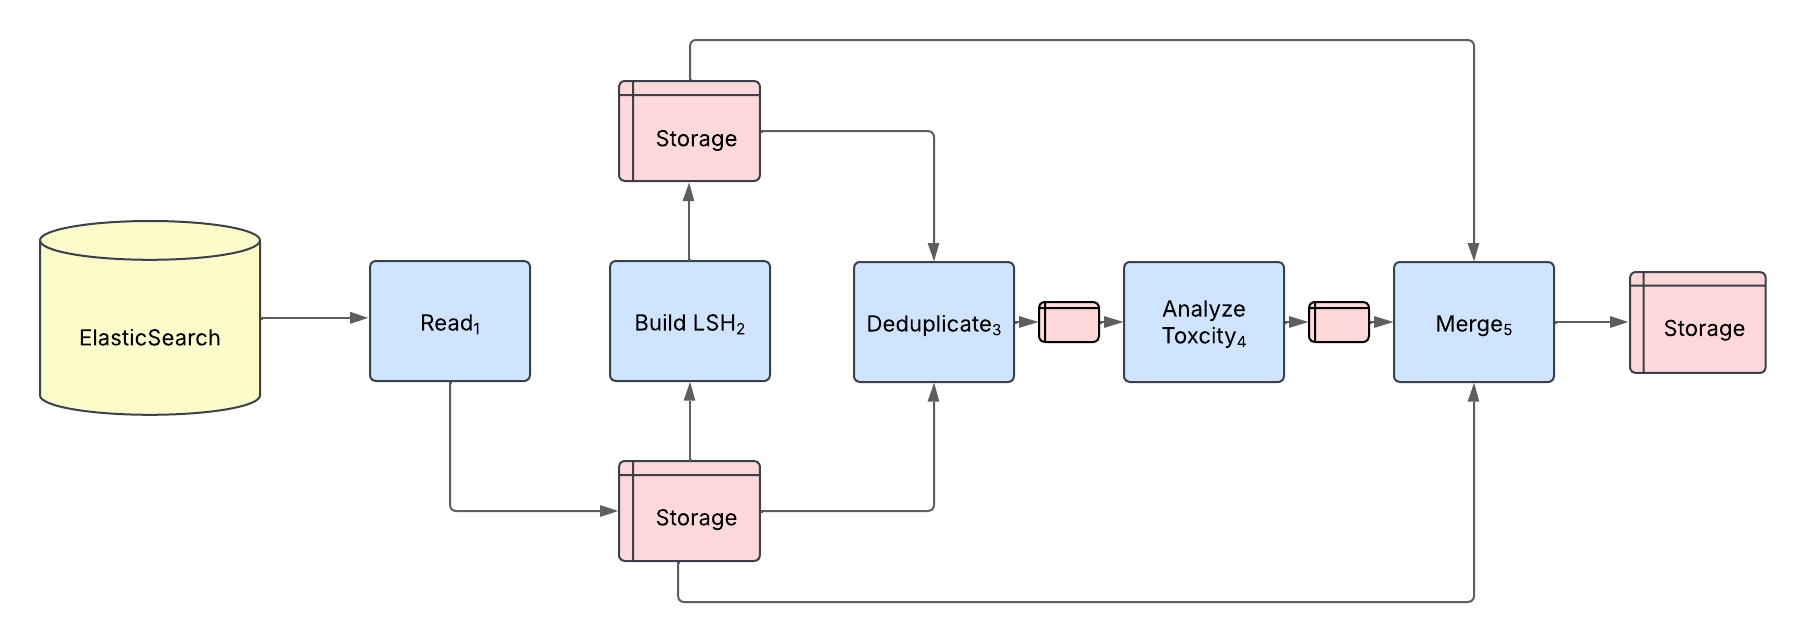
\includegraphics[width=\textwidth]{../material/pipeline.png}
    \caption{Data processing pipeline: 
    (\hyperref[step:reading]{1}) \textbf{Read}: Reading data from the ElasticSearch database; 
    (\hyperref[step:preprocess]{2}) \textbf{Preprocess}: Extracting plaintext and calculating MinHash (optional building subset); 
    (\hyperref[step:lsh]{3}) \textbf{Build LSH}: Building LSH index from processed data; 
    (\hyperref[step:dedup]{4}) \textbf{Deduplicate}: Near-duplicates are removed from processed data using the LSH index; 
    (\hyperref[step:toxicity]{5}) \textbf{Analyze Toxicity}: Performing toxicity analysis on deduplicated data; 
    (\hyperref[step:merge]{6}) \textbf{Merge}: Merging analyzed data with the original dataset using the LSH index. 
    Blue boxes represent processes, red indicates storage components, and yellow marks the external database.}
    \label{fig:pipeline}
\end{figure}

\paragraph{Reading Toots from Elasticsearch}\label{step:reading}
The pipeline's first stage retrieves the Mastodon data fields (described in Table~\ref{dataset-fields}) from Elasticsearch, applying the following filters:

\begin{enumerate}
    \item \textbf{Temporal scope}: Only toots posted during 2024
    \item \textbf{Instance selection}: From 1,000 fully crawled instances
    \item \textbf{Content filters}:
    \begin{itemize}
        \item \textbf{Original toots only} (excluding reblogs/boosts): \\
        Reblogs (boosts) were removed because only the ID and URL of the boosted toot are stored, not the original content. Fetching this content separately would introduce unnecessary complexity.
        
        \item \textbf{Text-only content} (removing toots with media attachments): \\ 
        Approximately~18\% of toots contain media attachments (mostly images). Since our toxicity detection models analyze only text, we excluded these toots to maintain consistency.
        
        \item \textbf{English-language labeled content}: \\
        Our analysis focuses on English-language toots to ensure compatibility with the toxicity models, which are optimized for English text.
    \end{itemize}
\end{enumerate}

We use the ray\_elasticsearch\footnote{\url{https://github.com/janheinrichmerker/ray-elasticsearch}} library for efficient Elasticsearch queries. The retrieved data contains the fields described in Table~\ref{dataset-fields}, including toot identifiers, content, instance information, and metadata flags. To avoid overloading the Elasticsearch cluster, we read data directly into local storage using the Parquet\footnote{\url{https://github.com/apache/parquet-java}} file format for efficient storage.

\paragraph{Language Detection using FastText}\label{step:language-detection}
Because the language labels provided by Mastodon are based on the users main language, there were still non-English toots in our subset. However, the detoxify unbiased model is only trained for English toxicity detection. To ensure only English texts are processed, a language detection step performed using the FastText\footnote{\url{https://huggingface.co/facebook/fasttext-language-identification}} model to predict each toot's language. We kept only those labeled as English for further analysis, thereby reducing the subset by approx 3 million toots and 205 instances, resulting in a final subset of 14,693,503 toots and 724 instances.
FastText is ideal for this task due to its use of subword information (character n-grams), which enables robust handling of informal language, misspellings, and slang common in social media texts. Its efficiency and accuracy in language detection ensure reliable filtering, even for short or noisy inputs \cite{joulin:2017}.

\subsection*{Handling Large Datasets by Minhash-based Deduplication and Merging}
Because of the high duplication rate of 95\% in the original dataset, we planned to deduplicate the data before analyzing it. After the analysis by our model we wanted to merge the results back into the original dataset. The deduplication and merging processes are based on MinHash signatures, which allow efficient identification of near-duplicate toots without having to compare every toot against each other in the dataset. In our actual analysis on the 1\% subset we directly analyzed the toots without deduplication and merging, because the subset contains less than 50\% duplicates and without the deduplication and merging our analysis was much faster. Nevertheless, we will explain the process here for future work.

\paragraph{Preperation for Minhash-based Deduplication and Merging}\label{step:preprocess} 
Before calculating the MinHash of every toot, the plaintext is extracted from the HTML content using the extract\_plain\_text function from resiliparse \cite{bevendorff:2018}. On the plaintext we can simply calculate the MinHash using the datasketch API\footnote{\url{https://ekzhu.com/datasketch/documentation.html\#minhash}}. The MinHash provides an efficient way to estimate the Jaccard similarity between documents. The Jaccard similarity $J(A,B)$ between two sets $A$ and $B$ is defined as:

\begin{equation}
J(A,B) = \frac{|A \cap B|}{|A \cup B|}
\end{equation}

MinHash works by computing multiple hash values for each document's shingles (contiguous subsequences of words) and keeping only the minimum hash value for each permutation. The probability that the minimum hash values match for two toots equals their Jaccard similarity \cite{broder:2000}. Our implementation uses 64 permutations to balance storage requirements with similarity estimation accuracy.

\subsubsection{LSH Index Construction}\label{step:lsh} 
The deduplication and merging employ Locality-Sensitive Hashing (LSH) techniques to efficiently identify and remove near-duplicate toots from the dataset \cite{leskovec:2014}. The idea of LSH is to group similar toots into buckets through a process called banding. This approach works by dividing each document's MinHash signature into $b$ bands of $r$ rows each. For a document with a MinHash signature of length $n$, we ensure $b \times r \le n$. Each band is then processed separately through a hash function, and toots sharing identical hash values in any band are considered potential duplicates. By setting the jaccard similarity threshold to 0.9, the optimizer finds values for $b$ and $r$ so that the probability of two toots sharing a band is very high when their Jaccard similarity is $\geq90\%$. The threshold is chosen to 0.9 because jaccard similarity is just indicating word similarity but not semantic similarity. To not remove toots that are similar in words but not in meaning, we suggest using a higher threshold than the maybe more realistic threshold of 0.58 explored by \citet{wu:2020} for similarity in short texts. 

We built one LSH index for the entire dataset. If this index gets queried, the responses are all toot id's matching a jaccard similarity $\geq90\%$ to the queried toot.

\paragraph{MinHash-based Similarity Deduplication}\label{step:dedup} 
For each toot we query the LSH index by inserting one toot's minhash and receving all similar ids in the same bucket. Within each group of near-duplicates, we retain only the toot with the smallest id value, ensuring deterministic selection while removing duplicates. This approach guarantees that only one representative instance of each near-duplicate group remains in the final dataset.

\paragraph{MinHash-based Similarity Merging}\label{step:merge}
The LSH index is queried for each toot in our subset to find similar toots. Because we kept the smallest id in the deduplication, now the smallest id in the query results always matches an id in the deduplicated dataset. We concatenate the matched analyzed toot from the deduplicated dataset with the original toot we used for our query. The toots now contain all relevant information and the the dataset for further analysis is created.

\section{Toxicity Analysis}\label{step:toxicity}
We used the detoxify unbiased model to perform zero-shot toxicity prediction on the 1\% subset. Zero-shot prediction means the model was not fine-tuned on Mastodon toots and makes predictions using only its pretrained knowledge. For each toot, the model predicts scores for all seven toxicity categories defined in Table~\ref{toxicity-categories}.

\begin{figure}[tb]
    \centering
    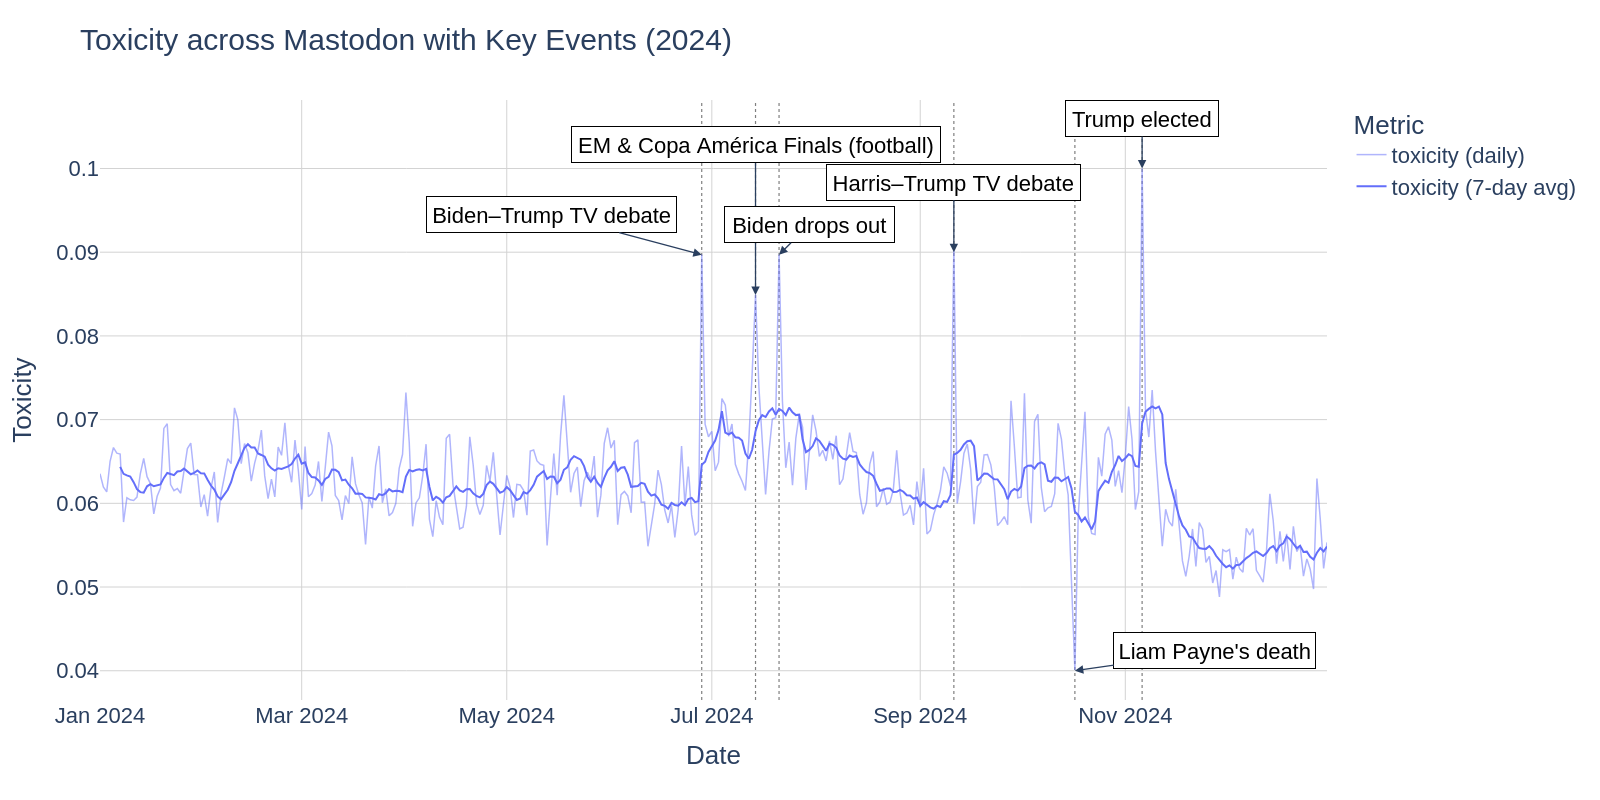
\includegraphics[width=\textwidth]{../material/toxicity_2024.png}
    \caption{Distribution of the daily mean value and a 7-day average for the toxicity category over the year~2024. The main peaks are marked with events that occurred on that day, which may have influenced the toxicity value.}
    \label{toxicity-2024}
\end{figure}

\subsection{Peak Analysis of Toxicity Timeline} 
Figure~\ref{toxicity-2024} shows the distribution of the daily mean value and a 7-day average for the toxicity category over the year~2024. Several peaks occur during major events, influencing the toxicity value. Overall, the toxicity value remains stable between 0.06 and 0.07 but drops toward the end of the year to 0.05. This drop may be explained by the increase in the total number of toots (Figure~\ref{toot-distribution}), indicating that toxic communities did not grow as much as non-toxic ones.

The most prominent peak coincides with the U.S. election results on November~6, 2024, when Donald Trump was elected president. The only clearly recognisable negative peak occurs on October~17, one day after Liam Payne's death. This peak likely results from a sudden increase in activity, with condolences and tributes eliciting positive sentiments. October~17 was the second most active day in 2024, probably due to the additional positive toots. Because it was a 'positive' rise, the mean toxicity level decreased in the end. Interestingly, the two days with the highest activity produced opposing toxicity peaks, as November~6 was the most active and most toxic day. 

Most peaks are related with key U.S. election events, possibly because the analysis focuses on English toots, and the majority of English speakers reside in the U.S. The largest non-election-related peak occurs on July~14, 2024, the day of the UEFA Euro~2024 and Copa América~2024 finals. Since this peak primarily falls under the threat category, it may reflect heightened aggression among football fans.

\subsection{Impact of Moderation Policies on Toxicity Levels}\label{moderation:categorization}

To explore the impact of moderation policies on toxicity levels, we scraped all instances linked in the picker from the Mastodon website\footnote{\url{https://joinmastodon.org/servers}}. All these instances committed to the Mastodon Covenant\footnote{\url{https://joinmastodon.org/covenant}}, which demands active moderation against racism, sexism, homophobia, and transphobia. Out of the 724 instances analyzed, 175 are part of the Mastodon Covenant. Following \citet{bono:2024} findings on blocklist-based moderation, we cross-referenced our instances with the \_unified\_tier0\_blocklist\footnote{\url{https://github.com/sgrigson/oliphant/blob/main/blocklists/README.md}} to uncover blocklisted instances from our crawl. Additionally we want to test whether toxicity is affected by communicating with blocklisted instances. We define \emph{communication} as occurring when users from blocklisted instances post on another instance.

We categorized the instances as follows to explore the impact of different moderation practices:
\begin{itemize}
\item \textbf{Moderated}: 175 Covenant instances (7,228,494 toots) representing explicit commitment to anti-toxicity policies.
\item \textbf{Blocklisted}: 13 blocklisted instances (92,403 toots) flagged by the community for harmful content, serving as a proxy for poorly moderated spaces.
\item \textbf{Communicating}: 286 instances (5,691,465 toots) communicating with blocklisted ones: Testing whether interaction with poorly moderated instances increases toxicity.
\item \textbf{Non-Communicating}: 250 instances (611,823 toots) not communicating with blocklisted ones: Providing a baseline for toxicity in isolated, but not Covenant-bound, communities.
\end{itemize}

\subsubsection{Formulating Hypotheses on How Moderation Policies Impact Toxicity}
We formulated four key hypotheses based on Mastodon's federated architecture and moderation mechanisms:

\begin{enumerate}
    \item \textbf{Moderated vs. Blocklisted:} \\
    We hypothesized that instances adhering to the Mastodon Covenant would show significantly lower toxicity scores than blocklisted instances. This expectation stems from the Covenant's explicit requirements for active moderation against racism, sexism, homophobia, and transphobia, while blocklisted instances represent spaces where such moderation is absent.

    \item \textbf{Moderated vs. Non-Communicating:} \\
    We expected no significant difference between toxicity scores in moderated and non-communicating instances, as both employ strategies to limit toxic content—either through active moderation or complete isolation from potentially toxic federated servers.

    \item \textbf{Communicating vs. Non-Communicating:} \\
    We hypothesized communicating instances to show higher toxicity scores than non-communicating ones, based on the premise that federation with poorly moderated servers allows toxic content to propagate through the network.

    \item \textbf{Blocklisted vs. Communicating:} \\
    We expected no significant difference between toxicity scores in blocklisted and communicating instances, as continuous interaction with toxic servers may lead to normalization and adoption of similar toxic behaviors.
\end{enumerate}


\subsubsection{Descriptive Analysis of Differences in Toxicity Scores Between Moderation Policies}

\begin{figure}[tb]
    \centering
    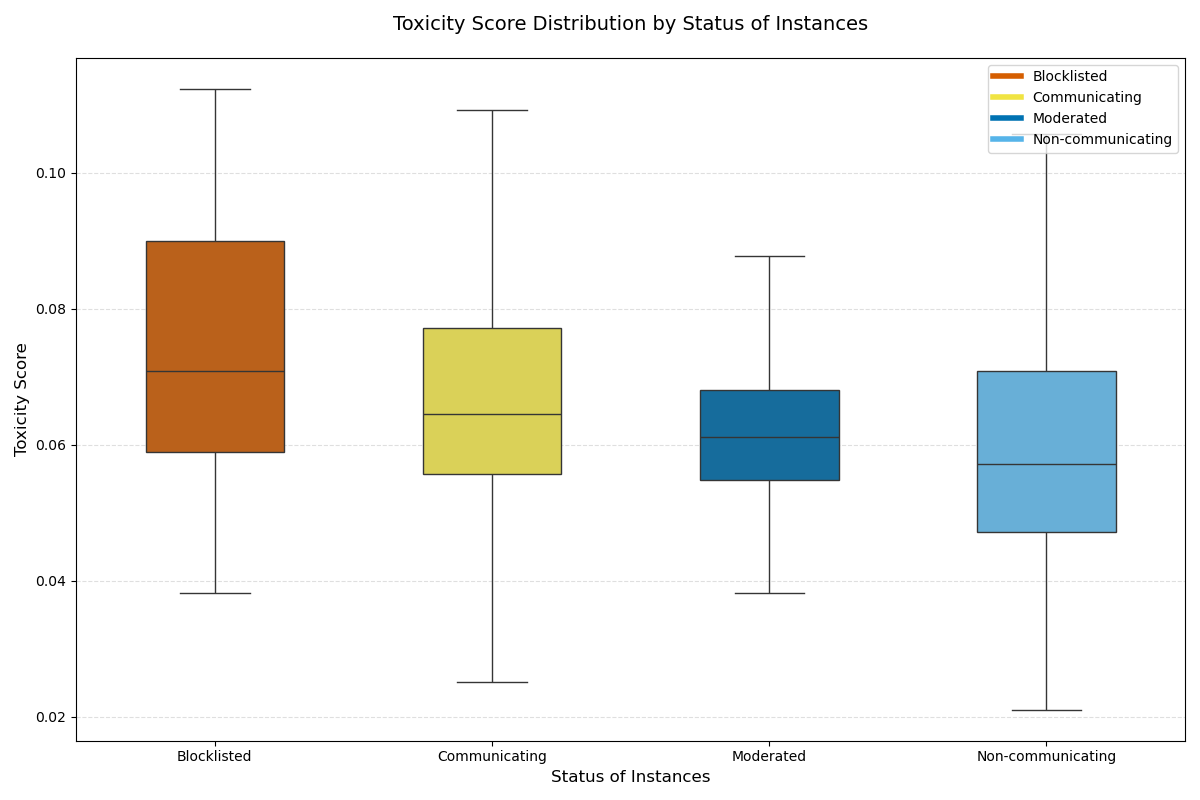
\includegraphics[width=\textwidth]{../material/blocklist_vs_covenant_boxplot.png}
    \caption{Comparison of average toxicity levels of instances across four instance categories: 
    \textbf{Blocklisted}: Instances flagged for spreading inappropriate content; 
    \textbf{Communicating}: Instances interacting with blocklisted instances; 
    \textbf{Moderated}: Mastodon Covenant members with active moderation policies;
    \textbf{Non-communicating}: Instances not interacting with any blocklisted instances.;
    The middle line marks the median, the box spans the IQR (25th–75th percentiles), and whiskers extend to 1.5×IQR.}
    \label{blocklisted-vs-covenant}
\end{figure}

 The results in Figure~\ref{blocklisted-vs-covenant} offer initial evidence that moderation practices influence toxicity levels. The plot reveals the distribution of toxicity scores across four types of Mastodon instances, categorized by their moderation policies. First the toxicity level of each instance is calculated by taking the mean score of all there crawled toots. Then each boxplot represents the average toxicity level per moderation policy, revealing clear differences in toxicity across categories.

\textbf{Blocklisted} instances demonstrate the highest toxicity levels, with a median toxicity score (Mdn = 0.072, M = 0.091, SD = 0.047) exceeding all other categories. The large interquartile range (IQR) reflects the small sample size in this category. Although those 13 instances can not be considered representative of all blocklisted instances, they show a clear trend of high toxicity.

\textbf{Moderated} instances following the Mastodon Covenant display lower toxicity levels overall. Their median toxicity score (Mdn = 0.061, M = 0.063, SD = 0.015) is only slightly above that of non-communicating instances, and their IQR is narrower than the others. The compact boxplot indicates that the instances in this category are likely to be more homogenous in their moderation practices. This suggests that instances adhering to the Mastodon Covenant and actively moderating their content result in a less toxic environment.

Instances \textbf{communicating} with blocklisted instances as well as \textbf{Non-communicating} instances display a broad IQR and large whiskers distance. Therefore the results should be viewed with caution. Due to the imprecise categorization based on the communication with blocklisted instances, insances likely differ in terms of toxicity level.

Nethertheless \textbf{communicating} instances show moderately elevated toxicity. While their median toxicity score (Mdn = 0.065, M = 0.069, SD = 0.022) falls below blocklisted instances, it remains higher than the other categories. This supports the assumption that interaction with blocklisted instances being supposed to moderate poorly lead to increased toxicity. 

\textbf{Non-communicating} instances even display the lowest median toxicity score (Mdn = 0.053, M = 0.057, SD = 0.045). Although this might not be a perfect categorization, the overall trend indicates these instances maintain less toxic environments, likely due to their isolation from blocklisted content.

These findings support our hypotheses that moderation policies and federation behavior impact toxicity levels. Instances implementing active moderation or isolating from toxic environments show lower toxicity, while those interacting with blocklisted instances demonstrate increased toxic content.

\subsubsection{Statistical Analysis of Toxicity Differences}
To statistically analyze these observations, we employed independent samples t-tests to evaluate mean differences in toxicity scores between instance categories. The t-test assesses whether the observed differences between categories are statistically significant (unlikely to occur by random chance), with $\alpha$ < .05 as significance threshold. To complement this, we calculated Cohen's d as a standardized measure of effect size, representing the magnitude of differences between categories independent of sample size. The results are summarized in Table~\ref{statistical-comparisons}.

\paragraph{Moderated vs. Blocklisted Instances}
The test reults confirmed our first hypothesis with statistically significant results ($t(14.26) = 2.264$, $p = .040$, $d = 1.40$) and a very large effect size. This substantial difference indicates that instances adhering to the Mastodon Covenant's moderation standards successfully maintain less toxic environments compared to blocklisted instances lacking such moderation.

\paragraph{Moderated vs. Non-Communicating Instances}
Contrary to our expectations, we found a statistically significant difference ($t(593.07) = 2.653$, $p = .008$, $d = 0.17$) between moderated and non-communicating instances, though with a small effect size. While significant, this minimal practical difference suggests our hypothesis about equivalent outcomes between these strategies requires refinement. The results imply that complete isolation from potentially toxic instances might be marginally more effective than relying solely on active content moderation.

\paragraph{Communicating vs. Non-Communicating Instances}
Our third hypothesis was strongly confirmed with highly significant results ($t(660.15) = 4.939$, $p < .001$, $d = 0.33$) and a small-to-medium effect size. This demonstrates that instances communicating with blocklisted servers exhibit noticeably higher toxicity levels than non-communicating instances. This result indicates that federation with blocklisted instances increases toxicity.

\paragraph{Blocklisted vs. Communicating Instances}
The statistical analysis failed to reject the null hypothesis ($t(14.30) = 1.784$, $p = .096$, $d=0.93$), indicating no significant difference in toxicity levels between blocklisted and communicating instances. While the observed means showed a descriptive difference, the lack of statistical significance means we cannot confidently conclude this represents a true population effect. This result leaves our hypothesis neither confirmed nor refuted - the data simply does not provide sufficient evidence to make a determination about the relationship between these instance types. The small sample size of blocklisted instances (n=13) particularly limits our ability to detect effects in this comparison.

\begin{table}[tb]
    \centering
    \begin{tabular}{@{}crrrrr@{}}
    \hline
    Comparison & t-statistic & df & p-value & Cohen's d & Effect Size \\
    \hline
    Moderated \\
    vs & 2.264 & 14.26 & \textbf{.040} & 1.40 & Very large \\
    Blocklisted \\
    \hline

    Moderated \\
    vs & 2.653 & 593.07 & \textbf{.008} & 0.17 & Small \\
    Non-communicating \\
    \hline

    Communicating \\
    vs & 4.940 & 660.15 & \textbf{<.001} & 0.33 & Medium \\
    Non-communicating \\
    \hline

    Moderated \\
    vs & 1.784 & 14.30 & .096 & 0.93 & Very large \\
    Communicating \\
    \hline
    \end{tabular}
    \caption{Summary of independent samples t-tests. Bold p-values indicate statistical significance ($\alpha$ < .05). Effect sizes interpreted using Cohen's d guidelines developed by \citet{funder:2019}.}
    \label{statistical-comparisons}
\end{table}

\chapter{Discussion} \label{discussion}

Our toxicity analysis revealed distinct patterns across Mastodon instances, aligning with the four categories we established based on moderation practices. The temporal analysis showed clear peaks in toxicity corresponding to major political and global events throughout 2024, particularly around the U.S. election period. The hierarchical distribution of toxicity levels—from highest in blocklisted instances to lowest in non-communicating ones—demonstrates a strong correlation between moderation practices and platform climate.

\paragraph{Interpretation of Results}
The results indicate that our toxicity prediction pipeline successfully captured meaningful patterns in the Mastodon dataset, despite limitations in model selection. The clear hierarchy of toxicity levels across instance categories supports our hypothesis that decentralized moderation practices significantly influence platform toxicity. The temporal peaks suggest that global events trigger increased toxic discourse, particularly in politically charged contexts. These findings validate our approach of using transformer-based models for large-scale toxicity analysis in federated social networks.

\paragraph{Comparison with Previous Work}
Our findings align with and extend previous research on decentralized moderation. \citet{bono:2024} observed widespread blocklist usage across Mastodon instances and raised concerns about potential misuse for moderating instances that may not require intervention. Our analysis demonstrates that blocklisted instances exhibit significantly higher mean toxicity levels, while instances not communicating with blocklisted content maintain the lowest toxicity. This evidence suggests that blocklists effectively moderate genuinely harmful instances when properly implemented. 

The temporal dimension of our analysis provides new insights into toxicity evolution during real-world events, complementing event-focused studies like \citet{fan:2022} on toxicity patterns during health crises.

\paragraph{Limitations}
Our study has several limitations that should be considered when interpreting the results.

\subparagraph{Model Selection}
We compared three toxicity detection models using a small labeled subset of 256 toots. While the F1 scores were suboptimal for all models, we prioritized prediction confidence, ultimately selecting the Detoxify Unbiased model. This small validation set may not fully represent the diversity of toxic content in our dataset. However, the model's performance in identifying toxicity trends across instances suggests it was suitable for our analysis goals.

\subparagraph{Data Scope}
The analysis used a 1\% subset (approximately 18 million toots) rather than the full dataset due to computational constraints. We omitted our planned deduplication and merging methods because the subset contained fewer duplicates (50\% versus 95\% in the full dataset). The LSH-based methods for deduplication and merging require optimization for full-dataset analysis, particularly regarding memory management during index queries.

\paragraph{Future Work}
Several promising directions emerge from this research:

First, analyzing the full dataset with optimized LSH methods would improve result reliability. The current 1\% subset, while substantial, loses information about small instances and may miss patterns visible only at full scale. Especially because the toxic instances are the smaller ones.

Second, exploring all seven toxicity labels from our model could reveal category-specific patterns. Our focus on overall toxicity provides a broad view, but deeper analysis of specific toxic behaviors (e.g., identity attacks versus threats) might yield more nuanced insights.

Third, there is an interesting pattern in the data that we could not analyze in this work. The number of toots marked as sensitive is very high on November~6, 2024, which is the day after the US election. This day is also the day with the highest toxicity prediction across all instances (Figure~\ref{sensitive-toots}). Sensitive labels are typically used by moderators to flag toxic content for removal. However, some sexually-oriented instances apply this label mainly for sexual content. When we focus on those with a significant increase in sensitive-labeled toots on November~6, 2024, the day of peak toxicity and sensitive-labeled toots, this approach helps distinguish moderation-related labeling from other uses. This could be done in future work to analyze this kind of moderation.




\chapter{Conclusion} \label{conclusion}


\appendix
\chapter{My First Appendix}
This was just missing.



% Bibliography
\bibliographystyle{plainnat} % requires package natbib. An alternative is apalike
\bibliography{literature}    % load file literature.bib

\end{document}

